\section{Modelo dinámico}
En esta sección se modelará el comportamiento de la arquitectura.
A diferencia de lo modelos  que se estudió en la sección anterior (diagramas
de bloques, diagrama de bloques internos) que hacen referencia al
\textit{qué} del sistema, en el modelado del comportamiento se
hace rerefenrencia al \textit{cómo} del sistema. Este \textit{cómo}
es descripto por el modelado del comportamiento dentro del
sistema \citep{HoltPery}.

En esta sección se verán diferentes 3 niveles de absatracción diferentes
de los modelos de comportamiento del sistema. En primer lugar, el
nivel más alto de abstracción es la máquina de estado, que considera la
interacción entre bloques. El siguiente diagrama que se verá es
el diagrama de secuencia, el cual pone en manifiesto los diferentes
mensajes que son enviadas entre las entidades. Y por último, se
desarrolla el diagrama de actividades, siendo este el nivel
más bajo de abstracción del modelado del comportamiento del sistema.

\subsection{Máquina de estado}
En esta subsección se describe el ciclo de vida de los
bloques que conforman la arquitectura. En resúmen, lo que se
pretende demostrar, es el compartamiento de los objetos de la
arquitectura.

En la Figura \ref{fig:StateMachineArqCompleta} se presenta la
máquina de estado de la arquitectura completa.  En esta se
puede observar todos los estados por los cuales la arquitectura
debe recorrer.

\begin{figure}[h!]
 \centering
 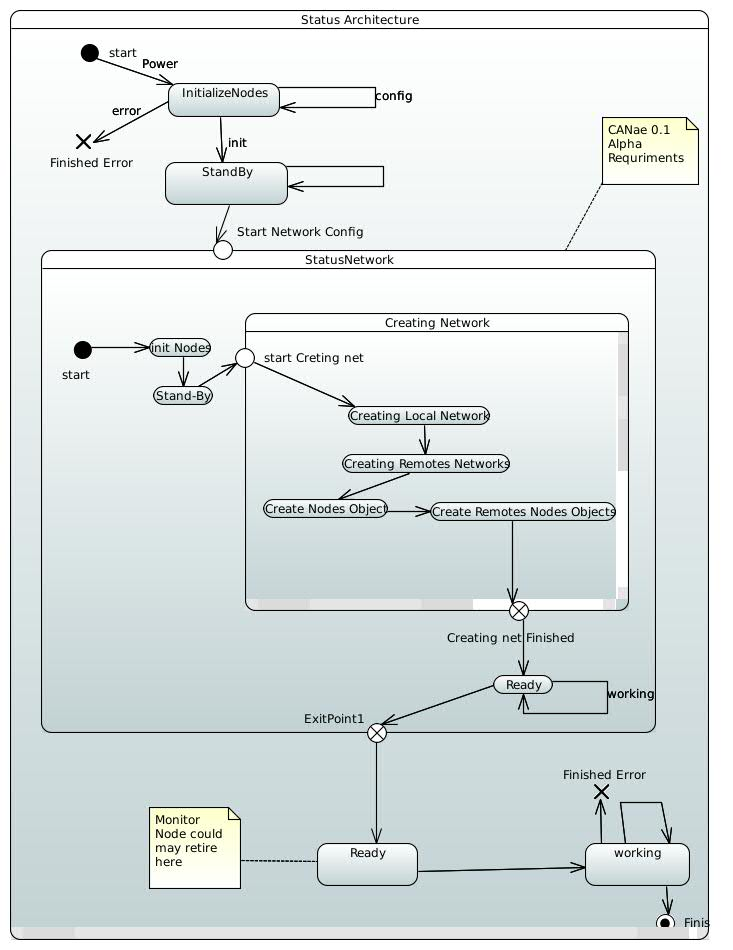
\includegraphics[scale=0.4]{images/Capitulo5/StateMachineArqCompleta.JPG}
  \caption{Máquina de estado de la arquitectura completa}
\label{fig:StateMachineArqCompleta}
\end{figure}

A continuación se procede a explicar la máquina de estado. Todo
inicia en el momento en el que la red es alimentada (eléctricamente)
siguiendo los protocolos de CAN \citep{can-ciaWEB}. En primer lugar, la
red pasa a un estdo de inicialización de los nodos, en los cuales, estos
son alimentados, se encienden, y comienzan con todos los procedimientos
normales de cualquier sistema embebido. Los cuales son Booteo, checkeo del
funcionamiento y del estado de salud del propio \ac{HW} y los \ac{HW}
conectados a él. Esto incluye la iniciación, del protocolo CANae como
un stack más del servicio del sistema operativo o sistema embebido
que gobierna a cada uno de los nodos. Esto se observa en la Figura
\ref{fig:StateMacineInitNodes}.

\begin{figure}[h!]
 \centering
 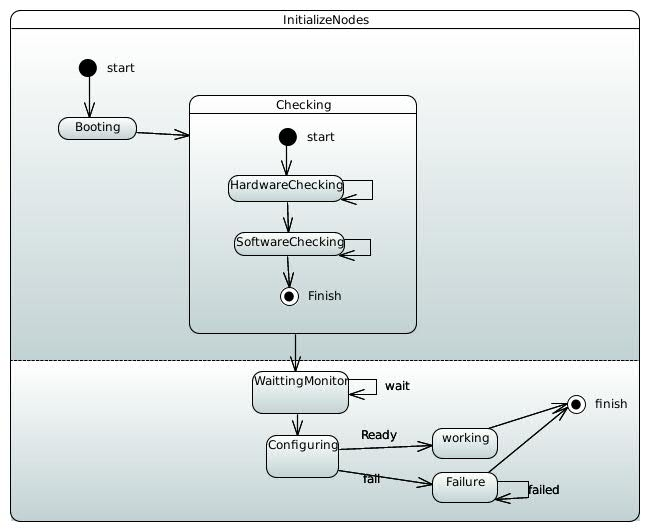
\includegraphics[scale=0.4]{images/Capitulo5/InitializeNodes.JPG}
  \caption{Máquina de estado de los nodos.}
\label{fig:StateMacineInitNodes}
\end{figure}

Una vez que todos los nodos se encuentran inicializados, y la red se encuentra
estable\footnote{Defínase como estable, la situación en la que el
  protocolo CANae se inicializó correctamente y está listo para pasar
  a la segunda etapa.}, la arquitectra pasa a un estado de Stand-By.
En este estado, la arquitectura espera por la orden del nodo monitor
para comenzar a configurar la red. Aquí se sigue lo indicado en el
protocolo CANae (Véase apéndice \ref{Appendix:A}). En primer lugar
el se crean las instancias de red localmente. Luego el nodo monitor
coordinar la creación de las instancias de red remota. Luego se crean
los objetos nodos tanto locales como remotos. Estas actividades
son necesarias para lograr entablecer una correcta comunicación
entre nodos utilizando el protocolo CANae (Versión 0.1 Alpha).

Una vez finalizada la creación de la red, la arquitectura completa
pasa a un estado Ready, donde el nodo monitor ya puede ser retirado.
Luego, la arquitectura ignora el nodo monitor (Si todavía se encuentra
conectado) y ya puede comenzar a trabajar normalmente.

\subsection{Diagrama de secuencia}
A continuación se muestra los diagramas de secuencias, para entender
cual es el comportamiento de la arquitectura, en un grado
de abstracción menor.

En la Figura \ref{fig:SecInitArq} se puede observar como en
el momento de alimentar (eléctricamente) a los nodos, este comienza
en primer lugar se ejecuta el boostrap. Este bootea al
sistema operativo (o sistema embebido según sea la tecnología
que se utilice). Una vez que el sistema operativo es cargado se
deben ejecutar (preferentemente) dos tipos diferentes de chequeos:
\begin{itemize}
\item Hardware Check
\item Software Check
\end{itemize}

\begin{figure}[h!]
 \centering
 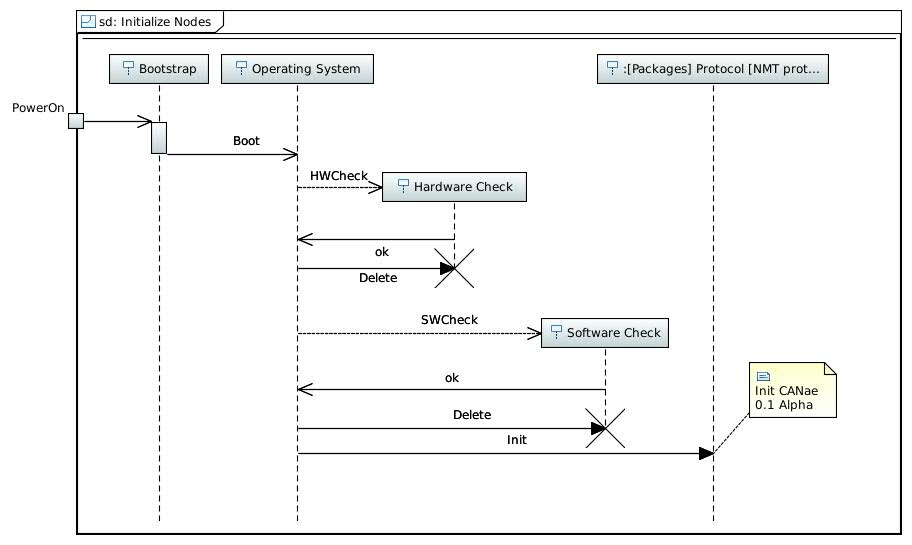
\includegraphics[scale=0.4]{images/Capitulo5/SecuenciaIInitNodes.JPG}
  \caption{Diagrama de secuencia del inicio de la arquitectura.}
\label{fig:SecInitArq}
\end{figure}

Estos son dos piezas de código. El primero tiene como tarea principal es
chequear el estado de salud de los equipos de hardware, tanto
del propio nodo, como así también del subsistema que tiene más proximo.
Como se expuso en la subsección \ref{subsec:bridge} cada nodo tiene
próximo a él (físicamente hablando) un subsistema (con su computadora
de vuelo). Por lo tanto el nodo se debe encargar de chequear el
estado de salud de los diferentes componetes de ese subsistema. El
segundo chequeo, se ocupa de verificar el estado de salud del software
tanto del nodo, como del subsistema más próximo.

Luego de que los chequeos se hayan resuelto exitosamente se crea una
instancia del protocolo CANae y da inicio a su servicio NMT. Este
servicio se puede observar en la Figura \ref{NMTC5}. En primer lugar
se debe esperar que el nodo monitor esté inicializado, y este les
envía un mensaje de \textit{crete\_remote\_network()} a todos los
nodos conectados a la arquitectura. Este mensaje llega al NMT del
protocolo de CANae de todos los nodos.

\begin{figure}[h!]
 \centering
 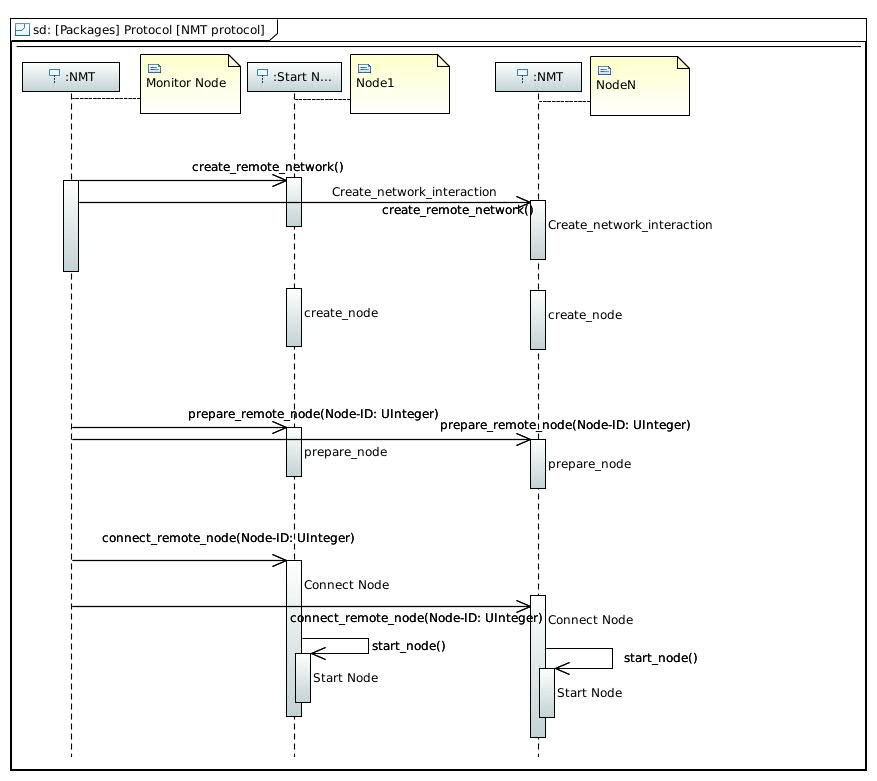
\includegraphics[scale=0.4]{images/Secciones/AppendixA/Protocol_NMT.JPG}
  \caption{Diagrama de secuencia de CA}
\label{fig:NMTC5}
\end{figure}

Luego, siguiendo el protocolo de CANae, cada nodo crea su instancia de
nodo. Esto puede observarse en la Figura \ref{fig:CreateNodeNMTC5}.
El objeto de \textit{CANAppLayerController} envía el mensaje \textit{
  create\_node()} al \textit{NodeManagement} de \textit{create\_newtork\_object()} con el objetivo de crear una instancia local de la red.


\begin{figure}[h!]
 \centering
 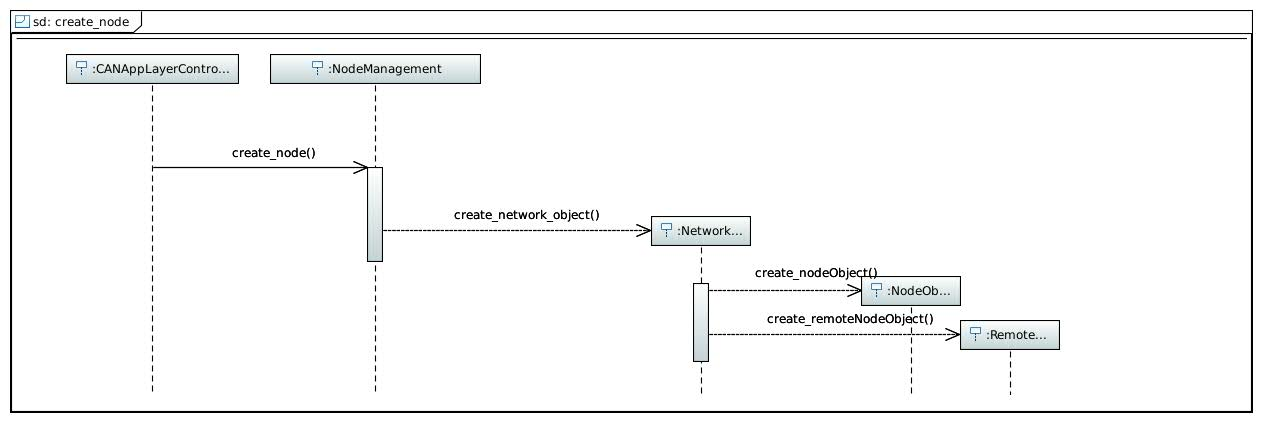
\includegraphics[scale=0.4]{images/Secciones/AppendixA/create_node.JPG}
  \caption{Crear Objecto Red, Objeto Nodo y Objeto Nodo Remoto}
  \label{fig:CreateNodeNMTC5}
\end{figure}

Luego el nodo monitor envía el mensaje \textit{prepare\_remote\_node}.
El protocolo CANae preve los pasos que se muestran en la Figura
\ref{fig:PrepareNodeC5}

\begin{figure}[h!]
 \centering
 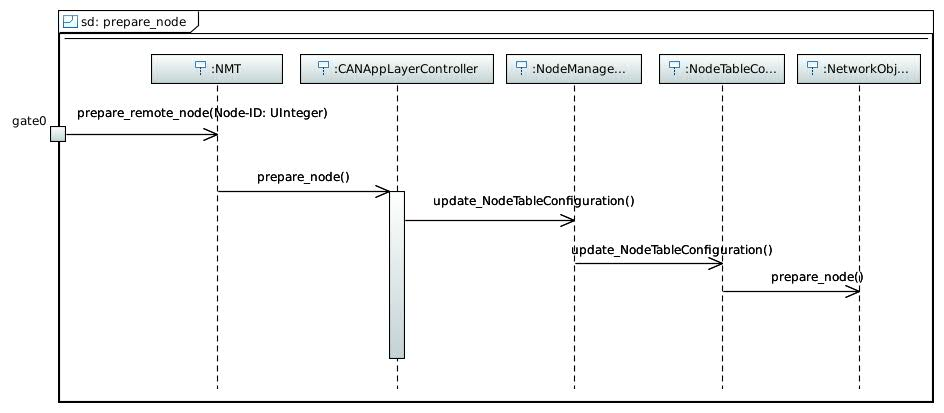
\includegraphics[scale=0.4]{images/Secciones/AppendixA/PrepareNode.JPG}
  \caption{Preparar nodo para la conexión a la red CAN}
  \label{fig:PrepareNodeC5}
\end{figure}

Por último, se conectan todo los nodos a la red, para lo cual deben
actualizar el \textit{Node Table Configuration}, y finalmente ya
ya pueden comenzar a comunicarse. Esto se observan en las Figuras
\ref{fig:PrepareNodeC5} y \ref{fig:ConnectNodeC5}

\begin{figure}[h!]
 \centering
 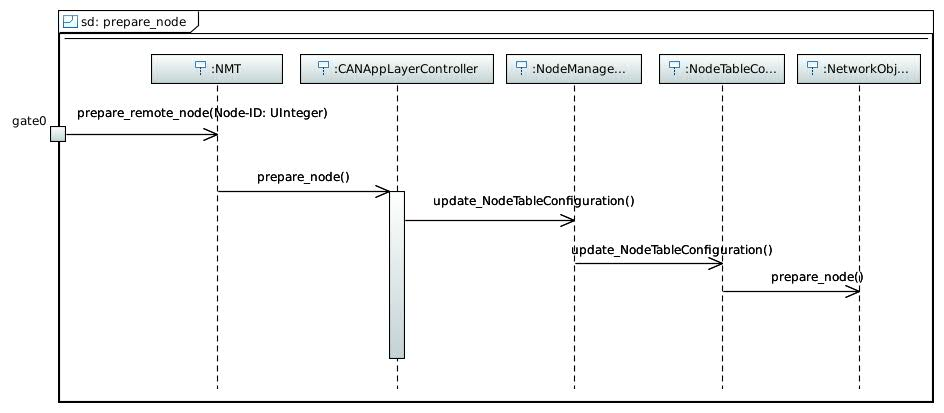
\includegraphics[scale=0.4]{images/Secciones/AppendixA/PrepareNode.JPG}
  \caption{Preparar nodo para la conexión a la red CAN}
  \label{fig:PrepareNodeC5}
\end{figure}

\begin{figure}[h!]
 \centering
 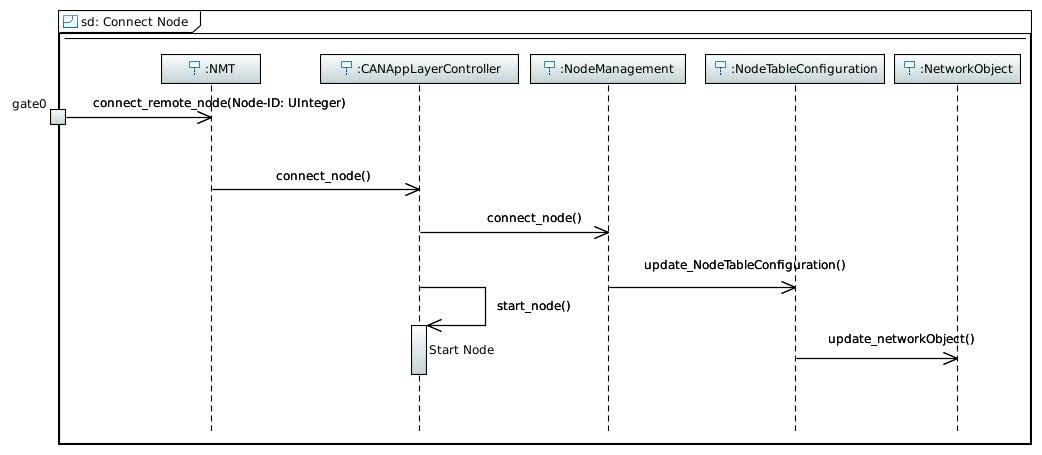
\includegraphics[scale=0.4]{images/Secciones/AppendixA/connect_node.JPG}
  \caption{Conectar el nodo a la red CAN}
  \label{fig:ConnectNodeC5}
\end{figure}

\subsection{Diagrama de actividades}






